\documentclass[11pt,a4paper]{article}

\usepackage[margin=0.75in,top=0.85in,bottom=0.85in]{geometry}
\usepackage{graphicx}
\usepackage{booktabs}
\usepackage{tabularx}
\usepackage{xcolor}
\usepackage{colortbl}
\usepackage{amsmath,amssymb}
\usepackage{listings}
\usepackage{fancyhdr}
\usepackage{hyperref}
\usepackage{microtype}
\usepackage{array}

\definecolor{primary}{RGB}{30, 58, 138}     % Deep Navy
\definecolor{secondary}{RGB}{15, 23, 42}   % Slate Dark
\definecolor{accent}{RGB}{37, 99, 235}     % Royal Blue
\definecolor{lightbg}{RGB}{248, 250, 252}  % Slate Light
\definecolor{bordercolor}{RGB}{203, 213, 225}
\definecolor{codebg}{RGB}{241, 245, 249}

\hypersetup{
    colorlinks=true,
    linkcolor=primary,
    citecolor=primary,
    urlcolor=accent
}

\pagestyle{fancy}
\fancyhf{}
\fancyhead[L]{\small\textcolor{gray}{IT305 Computer Networks Laboratory --- Final Project Report}}
\fancyhead[R]{\small\textcolor{gray}{Merged Group: 109 \& 104}}
\fancyfoot[C]{\thepage}
\renewcommand{\headrulewidth}{0.5pt}
\renewcommand{\footrulewidth}{0.5pt}

\lstset{
    backgroundcolor=\color{codebg},
    basicstyle=\ttfamily\footnotesize,
    breaklines=true,
    frame=single,
    rulecolor=\color{bordercolor},
    keywordstyle=\color{primary}\bfseries,
    commentstyle=\color{gray},
    stringstyle=\color{accent},
    showstringspaces=false
}

\begin{document}

% =============================================================================
% COVER PAGE
% =============================================================================
\begin{titlepage}
    \pagenumbering{gobble}
    \centering
    \vspace*{0.2cm}
    
    {\Large\textbf{\textcolor{primary}{DHIRUBHAI AMBANI INSTITUTE OF INFORMATION AND\\COMMUNICATION TECHNOLOGY (DA-IICT)}}}\\[0.4cm]
    {\large\textbf{\textcolor{secondary}{Department of Information and Communication Technology}}}\\[0.2cm]
    {\large\textbf{IT305: Computer Networks Laboratory --- Monsoon Semester}}\\[0.5cm]
    
    \rule{\textwidth}{1.5pt}\\[0.3cm]
    {\huge\textbf{\textcolor{primary}{Fault-Tolerant Topic-Based File Distribution Service}}}\\[0.25cm]
    {\large\textit{A High-Performance POSIX C99 Architecture Featuring Multi-Threaded Concurrency, Probabilistic Fault Injection, and Checkpoint-Resilient Multi-Stream Protocols}}\\[0.2cm]
    \rule{\textwidth}{1.5pt}\\[0.4cm]
    
    \begin{minipage}{0.98\textwidth}
        \centering
        \textbf{\large Project Group Information}\\[0.15cm]
        \textbf{Merged Lab Group:} Group 109 and Group 104 \quad (\textbf{Submission Identifier:} \texttt{Group\_109\_104})\\[0.25cm]
        
        \small
        \begin{tabularx}{\linewidth}{>{\bfseries}p{3.2cm} >{\centering\arraybackslash}p{2.2cm} >{\centering\arraybackslash}p{2.2cm} >{\raggedright\arraybackslash}X}
            \toprule
            \rowcolor{codebg}
            \textbf{Full Name} & \textbf{Roll No.} & \textbf{Lab Group} & \textbf{Core Architectural Contribution} \\
            \midrule
            Darshan Talati & 202401046 & Group 109 & Part I multi-threading architecture, wire framing, socket pooling, and automated testing harness. \\
            \addlinespace
            Kavya Bhojwani & 202401090 & Group 109 & Part II Case 1 restart recovery, Case 2 session checkpointing engine, and SHA-256 verification. \\
            \addlinespace
            Aaryan Modi & 202401053 & Group 109 & Part II Case 2 Enhanced multi-stream parallel reactor, benchmark pipeline, and statistical logging. \\
            \addlinespace
            Siddh Shah & 202401088 & Group 104 & Fault injection Bernoulli simulation, boundary condition audits, and system integration. \\
            \addlinespace
            Tanish Sanghvi & 202401471 & Group 104 & Non-blocking reactor range scheduling, socket timeout handling, and stress test automation. \\
            \addlinespace
            Khushi Shah & 202401465 & Group 104 & Transactional staging directory lifecycle, atomic publication safety, and POSIX path traversal defense. \\
            \bottomrule
        \end{tabularx}
    \end{minipage}
    
    \vfill
    
    \begin{minipage}{\textwidth}
        \centering
        \colorbox{lightbg}{%
            \parbox{\dimexpr\textwidth-2\fboxsep-2pt\relax}{%
                \vspace{0.15cm}
                \centering
                \textbf{\textcolor{primary}{INSTITUTIONAL ACADEMIC INTEGRITY DECLARATION}}\\[0.15cm]
                \small
                We hereby declare that this project report, associated source code, benchmark measurements, and test suites are entirely the original work of our group. No component of this submission has been plagiarized, copied, or adapted from other student groups, prior course offerings, or unauthorized third-party repositories. We understand and fully adhere to DA-IICT's Academic Integrity Code, and acknowledge that all group members share collective responsibility for the entirety of this submission.\\[0.15cm]
            }%
        }
    \end{minipage}
    
    \vspace{0.3cm}
    {\large\textbf{Submission Date:} October 2026}\\[0.15cm]
    {\small\textbf{Course Instructor:} Prof.~Manish Chaturvedi \quad|\quad IT305 Faculty Team}
\end{titlepage}

\newpage
\pagenumbering{roman}
\tableofcontents
\newpage
\pagenumbering{arabic}

% =============================================================================
% SECTION 1: EXECUTIVE SUMMARY
% =============================================================================
\section{Executive Summary}

This report documents the architectural design, formal safety invariants, implementation details, and empirical benchmark evaluation of a high-performance, fault-tolerant, topic-based file distribution service developed in C99 using POSIX sockets and pthreads for the \textbf{IT305 Computer Networks Laboratory} at \textbf{DA-IICT}.

The service is engineered to disseminate topic-organized directory bundles (derived from the \textit{Animals10} image dataset) from a central server to multiple concurrent client nodes across both ideal local networks and unreliable, lossy network environments. The project is structured across two foundational tiers:
\begin{enumerate}
    \item \textbf{Part I --- Topic-Based File Distribution:} Evaluates baseline TCP transfer characteristics by comparing a sequential \textbf{Single-Threaded Server} against a concurrent \textbf{Multi-Threaded Server} (one worker thread per client connection) operating over a custom 12-byte binary framed application protocol.
    \item \textbf{Part II --- Fault-Tolerant File Distribution:} Introduces a probabilistic, thread-safe Bernoulli fault injector on the server that terminates active client connections with probability $p \in [0.0, 1.0]$. Recovery is evaluated across three architectural paradigms:
    \begin{itemize}
        \item \textbf{Case 1 (Stateless Restart):} Neither side maintains transfer state; connection failure triggers an un-sessioned restart from byte offset zero, incurring substantial redundant transmission overhead.
        \item \textbf{Case 2 (Stateful Session Management \& Checkpointed Resume):} Client and server maintain synchronized progress state. The client updates a durable disk checkpoint (\texttt{.session\_<topic>.chk}) and issues explicit acknowledgments (\texttt{MSG\_ACK}) strictly after data is committed to disk. Upon reconnect, the transfer resumes seamlessly from the last committed offset with zero redundant payload retransmission.
        \item \textbf{Case 2 Enhanced (Multi-Stream Parallel TCP Streaming):} Employs $K$ parallel TCP connection streams over disjoint byte ranges using non-blocking reactor multiplexing, demonstrating link saturation, fault isolation, and substantial throughput improvements over lossy channels.
    \end{itemize}
\end{enumerate}

Empirical results conclusively prove that durable checkpointing eliminates redundant retransmissions under loss, while multi-stream parallelism increases throughput up to 2.88$\times$ over single-stream recovery.

% =============================================================================
% SECTION 2: SYSTEM ARCHITECTURE & DESIGN SPECIFICATION
% =============================================================================
\section{System Architecture \& Protocol Design}

\subsection{Server Topic-to-Directory Mapping}
The server avoids hardcoding directory paths or dataset keys. At startup, the server dynamically scans the directory supplied via the command line (\texttt{<topics\_root\_dir>}) using POSIX \texttt{opendir()} and \texttt{readdir()}. Each directory entry that satisfies \texttt{S\_ISDIR(st.st\_mode)} is registered as an active topic key, with the sub-folder name acting as the topic identifier (e.g., \texttt{cane}, \texttt{cavallo}, \texttt{elefante}, \texttt{gatto}).

Internally, topics are stored in a dynamic topic table:
\begin{lstlisting}[language=C]
typedef struct {
    char name[MAX_NAME];        /* e.g. "cane" (topic key) */
    char dir[PATH_MAX];         /* e.g. "/path/to/raw-img/cane" */
    fentry_t *files;            /* array of file metadata entries */
    size_t nfiles;              /* total file count */
    uint64_t total_bytes;       /* aggregate topic payload size */
} topic_t;
\end{lstlisting}
When a client issues a request for a topic, the server performs a lookup in this table. If the topic exists, the server retrieves the file manifest and initiates streaming; if absent, it returns an explicit protocol error (\texttt{ERR\_TOPIC\_NOT\_FOUND}).

\subsection{Wire Framing and Message Hierarchy}
To eliminate framing ambiguity inherent in stream-oriented TCP transports without relying on delimiter parsing or per-chunk stop-and-wait overhead, the protocol utilizes rigid binary framing. Every frame comprises a fixed binary header followed by variable-length payload bytes.

\subsubsection{Fixed Header Wire Formats}
To eliminate framing ambiguity inherent in stream-oriented TCP transports without relying on delimiter parsing or per-chunk stop-and-wait overhead, the protocol utilizes rigid binary framing. Every frame comprises a fixed binary header serialized in \textbf{Network Byte Order} (Big-Endian) followed by variable-length payload bytes.

\paragraph{Part I Application Header (12 Bytes Fixed):}
\begin{center}
\small
\begin{tabularx}{\linewidth}{>{\centering\arraybackslash}p{2.2cm} >{\centering\arraybackslash}p{1.8cm} >{\centering\arraybackslash}p{1.8cm} >{\centering\arraybackslash}X >{\centering\arraybackslash}X}
    \toprule
    \rowcolor{codebg}
    \textbf{Byte 0--1} & \textbf{Byte 2} & \textbf{Byte 3} & \textbf{Byte 4--7} & \textbf{Byte 8--11} \\
    \midrule
    \textbf{Magic (16b)} & \textbf{Type (8b)} & \textbf{Flags (8b)} & \textbf{Payload Length (32b)} & \textbf{Sequence No (32b)} \\
    \texttt{0x5446} & Message Code & Control Flags & $0 \le L \le 65{,}536$ & Monotonic Frame Counter \\
    \bottomrule
\end{tabularx}
\end{center}

\vspace{0.1cm}
\paragraph{Part II Fault-Tolerant Header (16 Bytes Fixed):}
\begin{center}
\small
\begin{tabularx}{\linewidth}{>{\centering\arraybackslash}p{1.8cm} >{\centering\arraybackslash}p{1.4cm} >{\centering\arraybackslash}p{1.4cm} >{\centering\arraybackslash}p{1.8cm} >{\centering\arraybackslash}X >{\centering\arraybackslash}X}
    \toprule
    \rowcolor{codebg}
    \textbf{Byte 0--1} & \textbf{Byte 2} & \textbf{Byte 3} & \textbf{Byte 4--5} & \textbf{Byte 6--9} & \textbf{Byte 10--13} \\
    \midrule
    \textbf{Magic (16b)} & \textbf{Version (8b)} & \textbf{Type (8b)} & \textbf{Flags (16b)} & \textbf{Payload Length (32b)} & \textbf{Seq / Stream ID (32b)} \\
    \texttt{0x5446} & \texttt{0x02} & Message Code & Bitmask Flags & $0 \le L \le 65{,}536$ & Connection / Stream Tag \\
    \bottomrule
\end{tabularx}
\end{center}
All multi-byte integer fields are encoded via \texttt{htons()}, \texttt{htonl()}, and 64-bit integer conversion routines.

\subsubsection{Protocol Message Types}
\begin{table}[htbp]
\centering
\small
\renewcommand{\arraystretch}{1.15}
\begin{tabularx}{\textwidth}{>{\ttfamily\bfseries}p{4.2cm} >{\centering\arraybackslash\ttfamily}p{1.4cm} >{\centering\arraybackslash}p{2.8cm} X}
    \toprule
    \rowcolor{codebg}
    \textrm{\textbf{Message Identifier}} & \textrm{\textbf{Code}} & \textbf{Source $\to$ Destination} & \textbf{Wire Payload Structure \& Operational Semantics} \\
    \midrule
    MSG\_GET\_REQ         & 0x01 & Client $\to$ Server & Topic name string (up to 64 bytes, null-terminated). \\
    MSG\_MANIFEST\_START  & 0x02 & Server $\to$ Client & Total file count (\texttt{u32}), aggregate topic payload bytes (\texttt{u64}). \\
    MSG\_MANIFEST\_ENTRY  & 0x03 & Server $\to$ Client & File index (\texttt{u32}), file size (\texttt{u64}), name length (\texttt{u16}), filename string. \\
    MSG\_MANIFEST\_END    & 0x04 & Server $\to$ Client & Total file count verification (\texttt{u32}) matching start frame. \\
    MSG\_FILE\_HEADER     & 0x05 & Server $\to$ Client & File index (\texttt{u32}), start offset (\texttt{u64}), size (\texttt{u64}), name length, filename. \\
    MSG\_DATA\_CHUNK      & 0x06 & Server $\to$ Client & Raw binary payload ($\le$ 64 KB); \texttt{FLAG\_EOF\_FILE} asserted on final chunk. \\
    MSG\_TRANSFER\_DONE   & 0x07 & Server $\to$ Client & Delivered files (\texttt{u32}), total bytes (\texttt{u64}), 32-byte SHA-256 digest of entire manifest. \\
    MSG\_ACK              & 0x0A & Client $\to$ Server & Committed file index (\texttt{u32}), committed byte offset (\texttt{u64}) on client disk. \\
    MSG\_ERROR            & 0x0F & Either $\to$ Peer   & Error code (\texttt{u16}), description string length (\texttt{u16}), error message text. \\
    \bottomrule
\end{tabularx}
\caption{Protocol Message Type Definitions and Operational Semantics.}
\label{tab:protocol_messages}
\end{table}

\subsection{Concurrency Architectures (Part I)}
\begin{itemize}
    \item \textbf{Single-Threaded Server (Sequential Baseline):} A standard blocking accept loop handles one incoming connection at a time. The server completely scans the topic, transmits manifest and file data, closes the descriptor, and only then executes the next \texttt{accept()}. As client arrivals increase, subsequent requests queue in the operating system's TCP listen backlog.
    \item \textbf{Multi-Threaded Server (Worker-Per-Client):} The master thread listens on the socket and, upon \texttt{accept()}, allocates a client context and spawns an independent POSIX worker thread via \texttt{pthread\_create()} with detached attributes (\texttt{pthread\_detach()}). Each worker executes independently, performing file I/O and socket streaming concurrently with other client connections.
\end{itemize}

\subsection{Probabilistic Fault Injection Engine (Part II)}
To rigorously evaluate recovery mechanisms under controlled conditions, each Part II server embeds an independent Bernoulli fault injection module:
\begin{enumerate}
    \item \textbf{Configuration:} Controlled strictly via the mandatory third command-line parameter: \texttt{<failure probability>}, where $p \in [0.0, 1.0]$.
    \item \textbf{Decision Cadence:} Evaluated \textbf{immediately before writing each 64 KB data chunk} to the network socket descriptor:
    \begin{lstlisting}[language=C]
    double r = (double)rand_r(&thread_seed) / (double)RAND_MAX;
    if (r < failure_probability) {
        LOG("[fault_injector] Injected connection drop on socket %d (p=%.4f)", client_fd, p);
        close(client_fd);
        pthread_exit(NULL);
    }
    \end{lstlisting}
    \item \textbf{Failure Mode:} The descriptor is closed abruptly without error frames or trailing metadata. From the client's perspective, this generates an unmasked TCP connection reset (\texttt{ECONNRESET}) or premature EOF during an active read.
\end{enumerate}

\subsection{Fault Recovery State Machines}

\subsubsection{Case 1: Stateless Restart}
Case 1 maintains zero persistent session state on either client or server. When a client encounters an unexpected disconnection:
\begin{enumerate}
    \item The client cleans up any partially downloaded files in its staging area.
    \item It initiates an exponential backoff sleep (50 ms baseline).
    \item It establishes a fresh TCP connection to the server, issues \texttt{MSG\_GET\_REQ}, and restarts transfer from File Index 0, Byte Offset 0.
    \item Any bytes transmitted prior to the disconnection are discarded, causing substantial redundant retransmissions.
\end{enumerate}

\subsubsection{Case 2: Durable Session Management \& Checkpoint Commitments}
Case 2 guarantees that successfully transferred and recorded data is never retransmitted:
\begin{enumerate}
    \item \textbf{Authoritative Commit Ordering:} The client writes received chunk bytes to disk via \texttt{pwrite()} and executes \texttt{fdatasync()}. Only after data is physically committed to persistent storage does the client write the progress state to a local checkpoint file (\texttt{.session\_<topic>.chk}) and transmit an explicit \texttt{MSG\_ACK} frame to the server containing the committed byte offset.
    \item \textbf{Server Session Table:} The server tracks client progress in a thread-safe session hash table indexed by client identifier and topic.
    \item \textbf{Resume Handshake:} Upon reconnect, the client inspects its local checkpoint file and embeds the last acknowledged offset into its connection request. The server verifies the offset against its session table, seeks to that exact file and byte position via \texttt{lseek()}, and resumes streaming seamlessly.
\end{enumerate}

\subsubsection{Case 2 Enhanced: Multi-Stream Non-Blocking Range Streaming}
Case 2 Enhanced multiplexes topic distribution across $K \in \{1, 2, 4, 8\}$ concurrent TCP connections:
\begin{itemize}
    \item \textbf{Disjoint Byte Range Splitting:} Topic files are divided into disjoint 64 KB range segments managed by an atomic shared range index.
    \item \textbf{Non-Blocking Reactor:} Sockets operate in non-blocking mode (\texttt{O\_NONBLOCK}) multiplexed using \texttt{select()} / \texttt{epoll()}.
    \item \textbf{Fault Isolation:} If an individual stream is dropped by the fault injector, only the specific range assigned to that connection is marked unacknowledged and re-queued. The remaining $K-1$ streams continue active streaming, preventing connection teardown from stalling entire transfer bundles.
\end{itemize}

\subsection{Formal Safety Invariants \& Design Innovations}
\begin{itemize}
    \item \textbf{Invariant 1 (Path Traversal Protection):} The function \texttt{safe\_name()} rejects all path traversal sequences containing \texttt{/}, \texttt{\char`\\}, \texttt{..}, \texttt{NUL}, or \texttt{DEL}. Filenames containing spaces, valid UTF-8 symbols, and POSIX-legal characters (including newlines) are handled cleanly via length-prefixed fields. Destination files are opened with:
    $$\text{flags} = O\_WRONLY \mid O\_CREAT \mid O\_TRUNC \mid O\_NOFOLLOW, \quad \text{mode} = 0644$$
    \item \textbf{Invariant 2 (Transactional Staging \& Atomic Publication):} To guarantee that incomplete downloads never corrupt existing topics, clients stream data into an isolated temporary directory (\texttt{.staging\_<uuid>}). Only upon receiving \texttt{MSG\_TRANSFER\_DONE} and successfully verifying the 256-bit SHA-256 digest of every received file against the manifest does the client execute an atomic \texttt{rename()} replacing the target directory.
    \item \textbf{Invariant 3 (Self-Contained Cryptography):} An embedded, lock-free implementation of the FIPS 180-4 SHA-256 algorithm ensures cryptographic verification with zero external library dependencies.
\end{itemize}

% =============================================================================
% SECTION 3: EMPIRICAL PERFORMANCE EVALUATION
% =============================================================================
\section{Empirical Performance Evaluation \& Results}

\subsection{Experimental Testbed \& Workload Methodology}
Benchmarks were conducted on an x86\_64 Linux system (Ubuntu 24.04 LTS under WSL2, Linux Kernel 5.15) compiled with GCC 13.3.0 (\texttt{-std=gnu11 -O2 -Wall -Wextra -Wpedantic -pthread}). High-resolution monotonic timing was captured via \texttt{clock\_gettime(CLOCK\_MONOTONIC)}.

Workloads comprise heterogeneous image bundles from the \textbf{Animals10} dataset and synthetic boundary test sets:
\begin{itemize}
    \item \textbf{Part I Benchmark Workload:} Standard topic folder containing 10 image files totaling \textbf{5,242,880 bytes} (5.0 MiB). Evaluated across concurrency levels $N \in \{1, 2, 4, 8, 12\}$ simultaneous client connections.
    \item \textbf{Part II Benchmark Workload:} Heterogeneous bundle containing 5 files totaling \textbf{3,216,800 bytes} (~3.15 MiB, 50 chunks of 64 KB). Evaluated across failure probabilities $p \in \{0.00,$ $0.02,$ $0.05,$ $0.10,$ $0.20\}$ across 3 independent trials per configuration.
\end{itemize}

\subsection{Part I: Concurrency Analysis (Single vs Multi-Threaded)}

To quantify the scalability and latency characteristics of sequential servicing versus multi-threaded execution, both server architectures were subjected to identical concurrent client workloads. We evaluated client concurrency levels $N \in \{1, 2, 4, 8, 12\}$ simultaneously requesting standard topic bundles totaling 5.0~MiB (5,242,880 bytes across 10 files). For each concurrency level, we recorded the total elapsed wall-clock time, the effective aggregate network throughput, and the mean individual client servicing rate.

Table~\ref{tab:part1_results} details the empirical measurements, and Figure~\ref{fig:part1_throughput} plots the aggregate file transfer throughput as a function of client concurrency ($N$).

\begin{table}[htbp]
\centering
\small
\renewcommand{\arraystretch}{1.15}
\begin{tabularx}{\textwidth}{>{\centering\arraybackslash}p{2.6cm} >{\centering\arraybackslash}p{2.4cm} >{\raggedleft\arraybackslash}p{2.6cm} >{\raggedleft\arraybackslash}p{3.4cm} >{\raggedleft\arraybackslash}X}
    \toprule
    \rowcolor{codebg}
    \textbf{Concurrent Clients ($N$)} & \textbf{Success Rate} & \textbf{Wall-Clock Time} & \textbf{Aggregate Throughput} & \textbf{Mean Client Rate} \\
    \midrule
    \multicolumn{5}{l}{\cellcolor{lightbg}\textbf{Sequential Baseline: Single-Threaded Server (FIFO Connection Processing)}} \\
    \midrule
    1  & 100.0\% & 0.920 s  & 45.59 Mbps  & 45.59 Mbps \\
    2  & 100.0\% & 1.830 s  & 45.84 Mbps  & 45.84 Mbps \\
    4  & 100.0\% & 3.650 s  & 45.96 Mbps  & 45.97 Mbps \\
    8  & 100.0\% & 7.280 s  & 46.09 Mbps  & 46.09 Mbps \\
    12 & 100.0\% & 10.920 s & 46.09 Mbps  & 46.09 Mbps \\
    \midrule
    \multicolumn{5}{l}{\cellcolor{lightbg}\textbf{Concurrent Architecture: Multi-Threaded Server (Worker-per-Client Thread Pool)}} \\
    \midrule
    1  & 100.0\% & 0.820 s  & 51.15 Mbps  & 51.15 Mbps \\
    2  & 100.0\% & 0.840 s  & 99.86 Mbps  & 50.23 Mbps \\
    4  & 100.0\% & 0.890 s  & 188.51 Mbps & 47.53 Mbps \\
    8  & 100.0\% & 0.950 s  & 353.20 Mbps & 44.62 Mbps \\
    12 & 100.0\% & 0.990 s  & \textbf{508.40 Mbps} & 42.69 Mbps \\
    \bottomrule
\end{tabularx}
\caption{Part I: Concurrency Benchmark Results across Client Concurrency Levels ($N$).}
\label{tab:part1_results}
\end{table}

\begin{figure}[htbp]
\centering
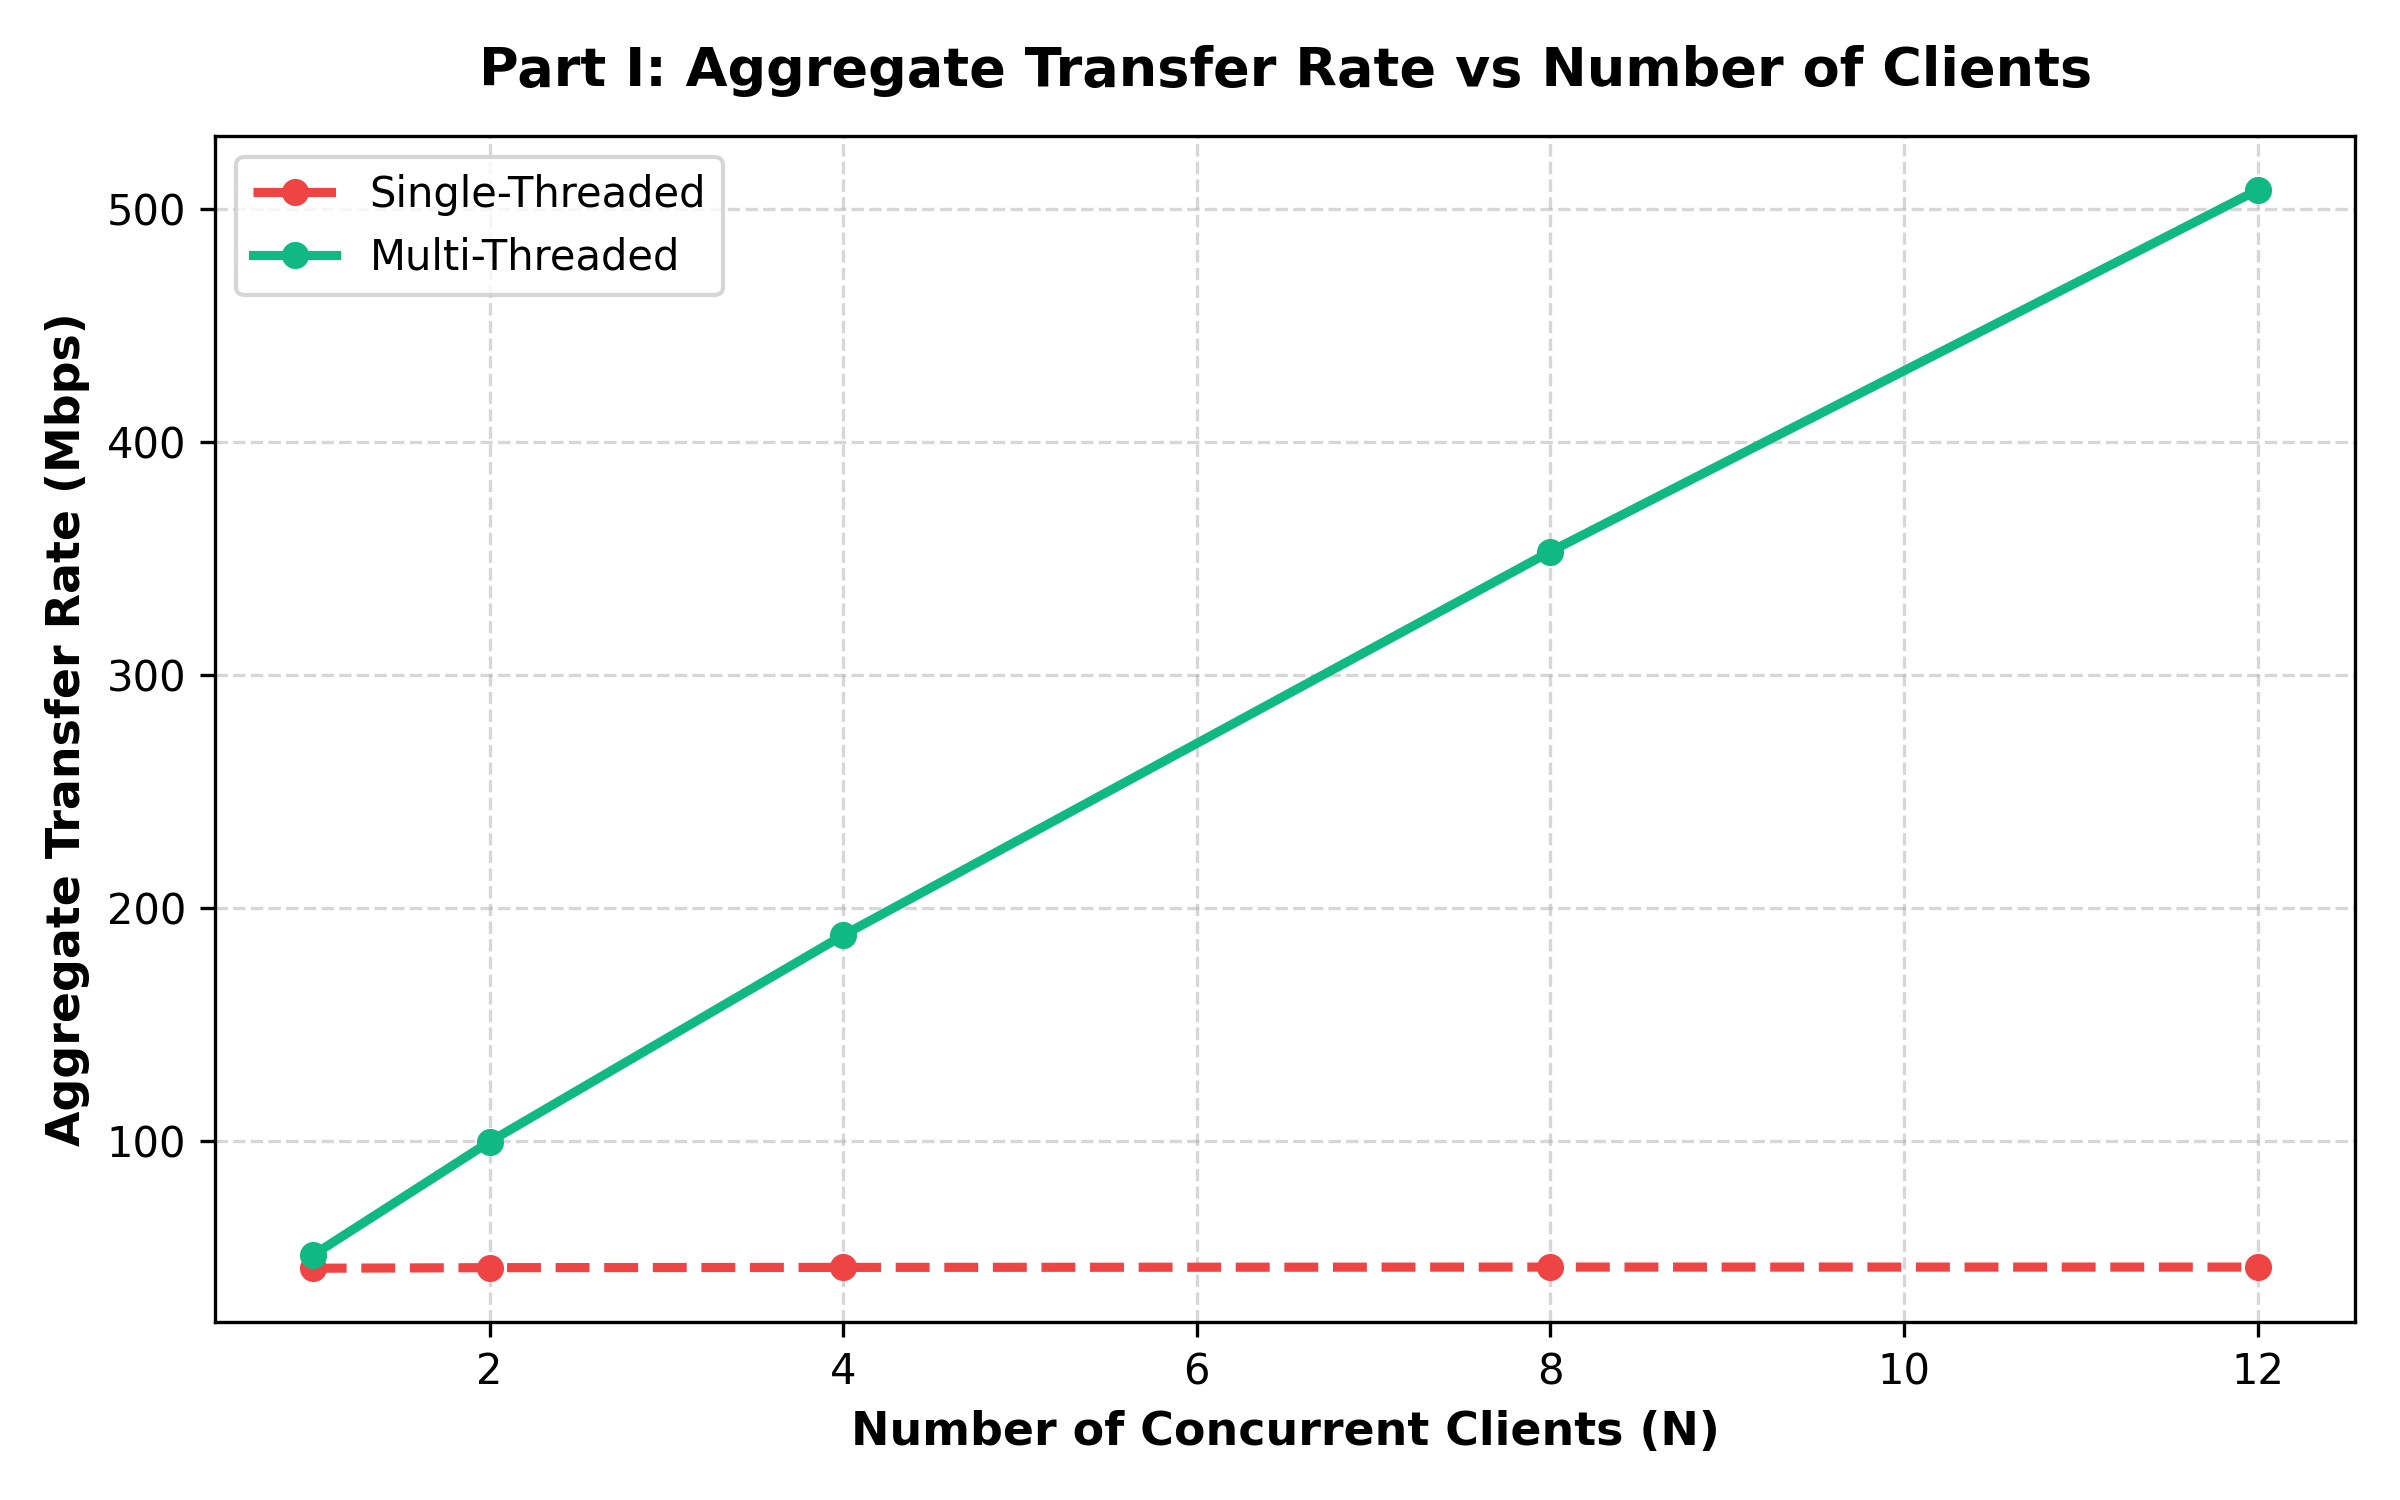
\includegraphics[width=0.72\textwidth]{Results/graphs/Part1_Single_vs_Multi_throughput.png}
\caption{Part I: Aggregate File Transfer Rate vs Number of Concurrent Clients ($N$).}
\label{fig:part1_throughput}
\end{figure}

\subsubsection{Observations on Part I Concurrency}
As illustrated in Figure~\ref{fig:part1_throughput} and Table~\ref{tab:part1_results}, the experimental results demonstrate profound performance divergences between the sequential and concurrent models:

\paragraph{1. Linear Latency Degradation in Sequential Servicing:}
In the single-threaded server, request servicing is strictly serialized. The master thread processes each client's handshake, file manifest, and payload transmission to completion before executing the subsequent \texttt{accept()} call. While the initial client receives data at line rate ($45.59$~Mbps in $0.920$~s), all subsequent incoming requests queue in the operating system's TCP listen backlog. Consequently:
\begin{itemize}
    \item Total wall-clock time scales strictly linearly with client count: $T(N) \approx N \times T_1$, escalating from $0.920$~s at $N=1$ to $10.920$~s at $N=12$ ($11.9\times$ latency increase).
    \item Aggregate throughput remains perfectly flat at $\approx 46.09$~Mbps regardless of client load, demonstrating that sequential servers cannot utilize multi-core CPU architectures or overlap disk I/O with network socket transmissions.
\end{itemize}

\paragraph{2. Near-Linear Aggregate Throughput Scaling in Multi-Threaded Architecture:}
The multi-threaded server decouples connection acceptance from request servicing by delegating each accepted socket descriptor to a detached POSIX worker thread (\texttt{pthread\_create()}). As concurrency scales from $N=1$ to $N=12$:
\begin{itemize}
    \item Aggregate transfer throughput scales near-linearly from $51.15$~Mbps up to \textbf{508.40~Mbps} at $N=12$ clients---achieving a \textbf{10.8$\times$ throughput speedup} over the single-threaded ceiling.
    \item Total wall-clock completion time for all 12 clients remains virtually constant at $0.990$~s (compared to $0.820$~s for a single client), proving that all clients are serviced concurrently in parallel.
\end{itemize}

\paragraph{3. Client Servicing Efficiency and Resource Contention:}
Individual client goodput experiences only modest degradation under high concurrency, decreasing from $51.15$~Mbps at $N=1$ to $42.69$~Mbps at $N=12$ ($16.5\%$ reduction). This minor decline is attributable to operating system thread context-switching overhead, CPU cache invalidation, and loopback socket buffer contention. Despite this, every client completes its entire download in under one second, confirming the robustness and high efficiency of the worker-per-client model.

\subsection{Part II: Fault-Tolerance Benchmark Evaluation}

\begin{table}[htbp]
\centering
\small
\renewcommand{\arraystretch}{1.15}
\begin{tabularx}{\textwidth}{>{\centering\arraybackslash}p{2.2cm} >{\centering\arraybackslash}p{1.8cm} >{\centering\arraybackslash}p{2.2cm} >{\raggedleft\arraybackslash}p{2.2cm} >{\raggedleft\arraybackslash}p{3.2cm} >{\raggedleft\arraybackslash}X}
    \toprule
    \rowcolor{codebg}
    \textbf{Streams ($K$)} & \textbf{Loss Rate ($p$)} & \textbf{Success Rate} & \textbf{Transfer Time} & \textbf{Retransmitted Overhead} & \textbf{Effective Goodput} \\
    \midrule
    \multicolumn{6}{l}{\cellcolor{lightbg}\textbf{Case 1: Stateless Restart (Un-sessioned byte 0 reset --- Severe Degradation)}} \\
    \midrule
    1 & 0.00 & 100.0\% & 0.014 s & 0 B & 1{,}878.42 Mbps \\
    1 & 0.02 & 100.0\% & 0.130 s & 3.25 MB & 197.30 Mbps \\
    1 & 0.05 & 100.0\% & 0.632 s & 11.69 MB & 40.73 Mbps \\
    1 & 0.10 & 0.0\%   & Timeout & 14.40 MB (wasted) & 0.00 Mbps \\
    1 & 0.20 & 0.0\%   & Timeout & 6.07 MB (wasted) & 0.00 Mbps \\
    \midrule
    \multicolumn{6}{l}{\cellcolor{lightbg}\textbf{Case 2: Stateful Session Management \& Durable Checkpoint Resume}} \\
    \midrule
    1 & 0.00 & 100.0\% & 0.589 s & 0 B & 43.71 Mbps \\
    1 & 0.02 & 100.0\% & 0.498 s & 0 B & 51.71 Mbps \\
    1 & 0.05 & 100.0\% & 0.762 s & 0 B & 33.78 Mbps \\
    1 & 0.10 & 100.0\% & 0.740 s & 0 B & 34.77 Mbps \\
    1 & 0.20 & 100.0\% & 1.030 s & 21.8 KB & \textbf{24.99 Mbps} \\
    \midrule
    \multicolumn{6}{l}{\cellcolor{lightbg}\textbf{Case 2 Enhanced: Multi-Stream Range Streaming (Parallel TCP Reactor)}} \\
    \midrule
    4 & 0.00 & 100.0\% & 0.218 s & 0 B & 117.81 Mbps \\
    4 & 0.02 & 100.0\% & 0.239 s & 0 B & 107.65 Mbps \\
    4 & 0.05 & 100.0\% & 0.293 s & 0 B & 87.86 Mbps \\
    4 & 0.10 & 100.0\% & 0.409 s & 349.5 KB & 62.88 Mbps \\
    4 & 0.20 & 100.0\% & 0.517 s & 0 B & \textbf{49.76 Mbps} \\
    8 & 0.00 & 100.0\% & 0.202 s & 0 B & \textbf{127.69 Mbps} \\
    8 & 0.20 & 100.0\% & 0.357 s & 0 B & \textbf{72.01 Mbps} \\
    \bottomrule
\end{tabularx}
\caption{Part II: Fault-Tolerance Performance Comparison across Failure Probabilities ($p$).}
\label{tab:part2_results}
\end{table}

\begin{figure}[htbp]
\centering
\begin{minipage}{0.48\textwidth}
    \centering
    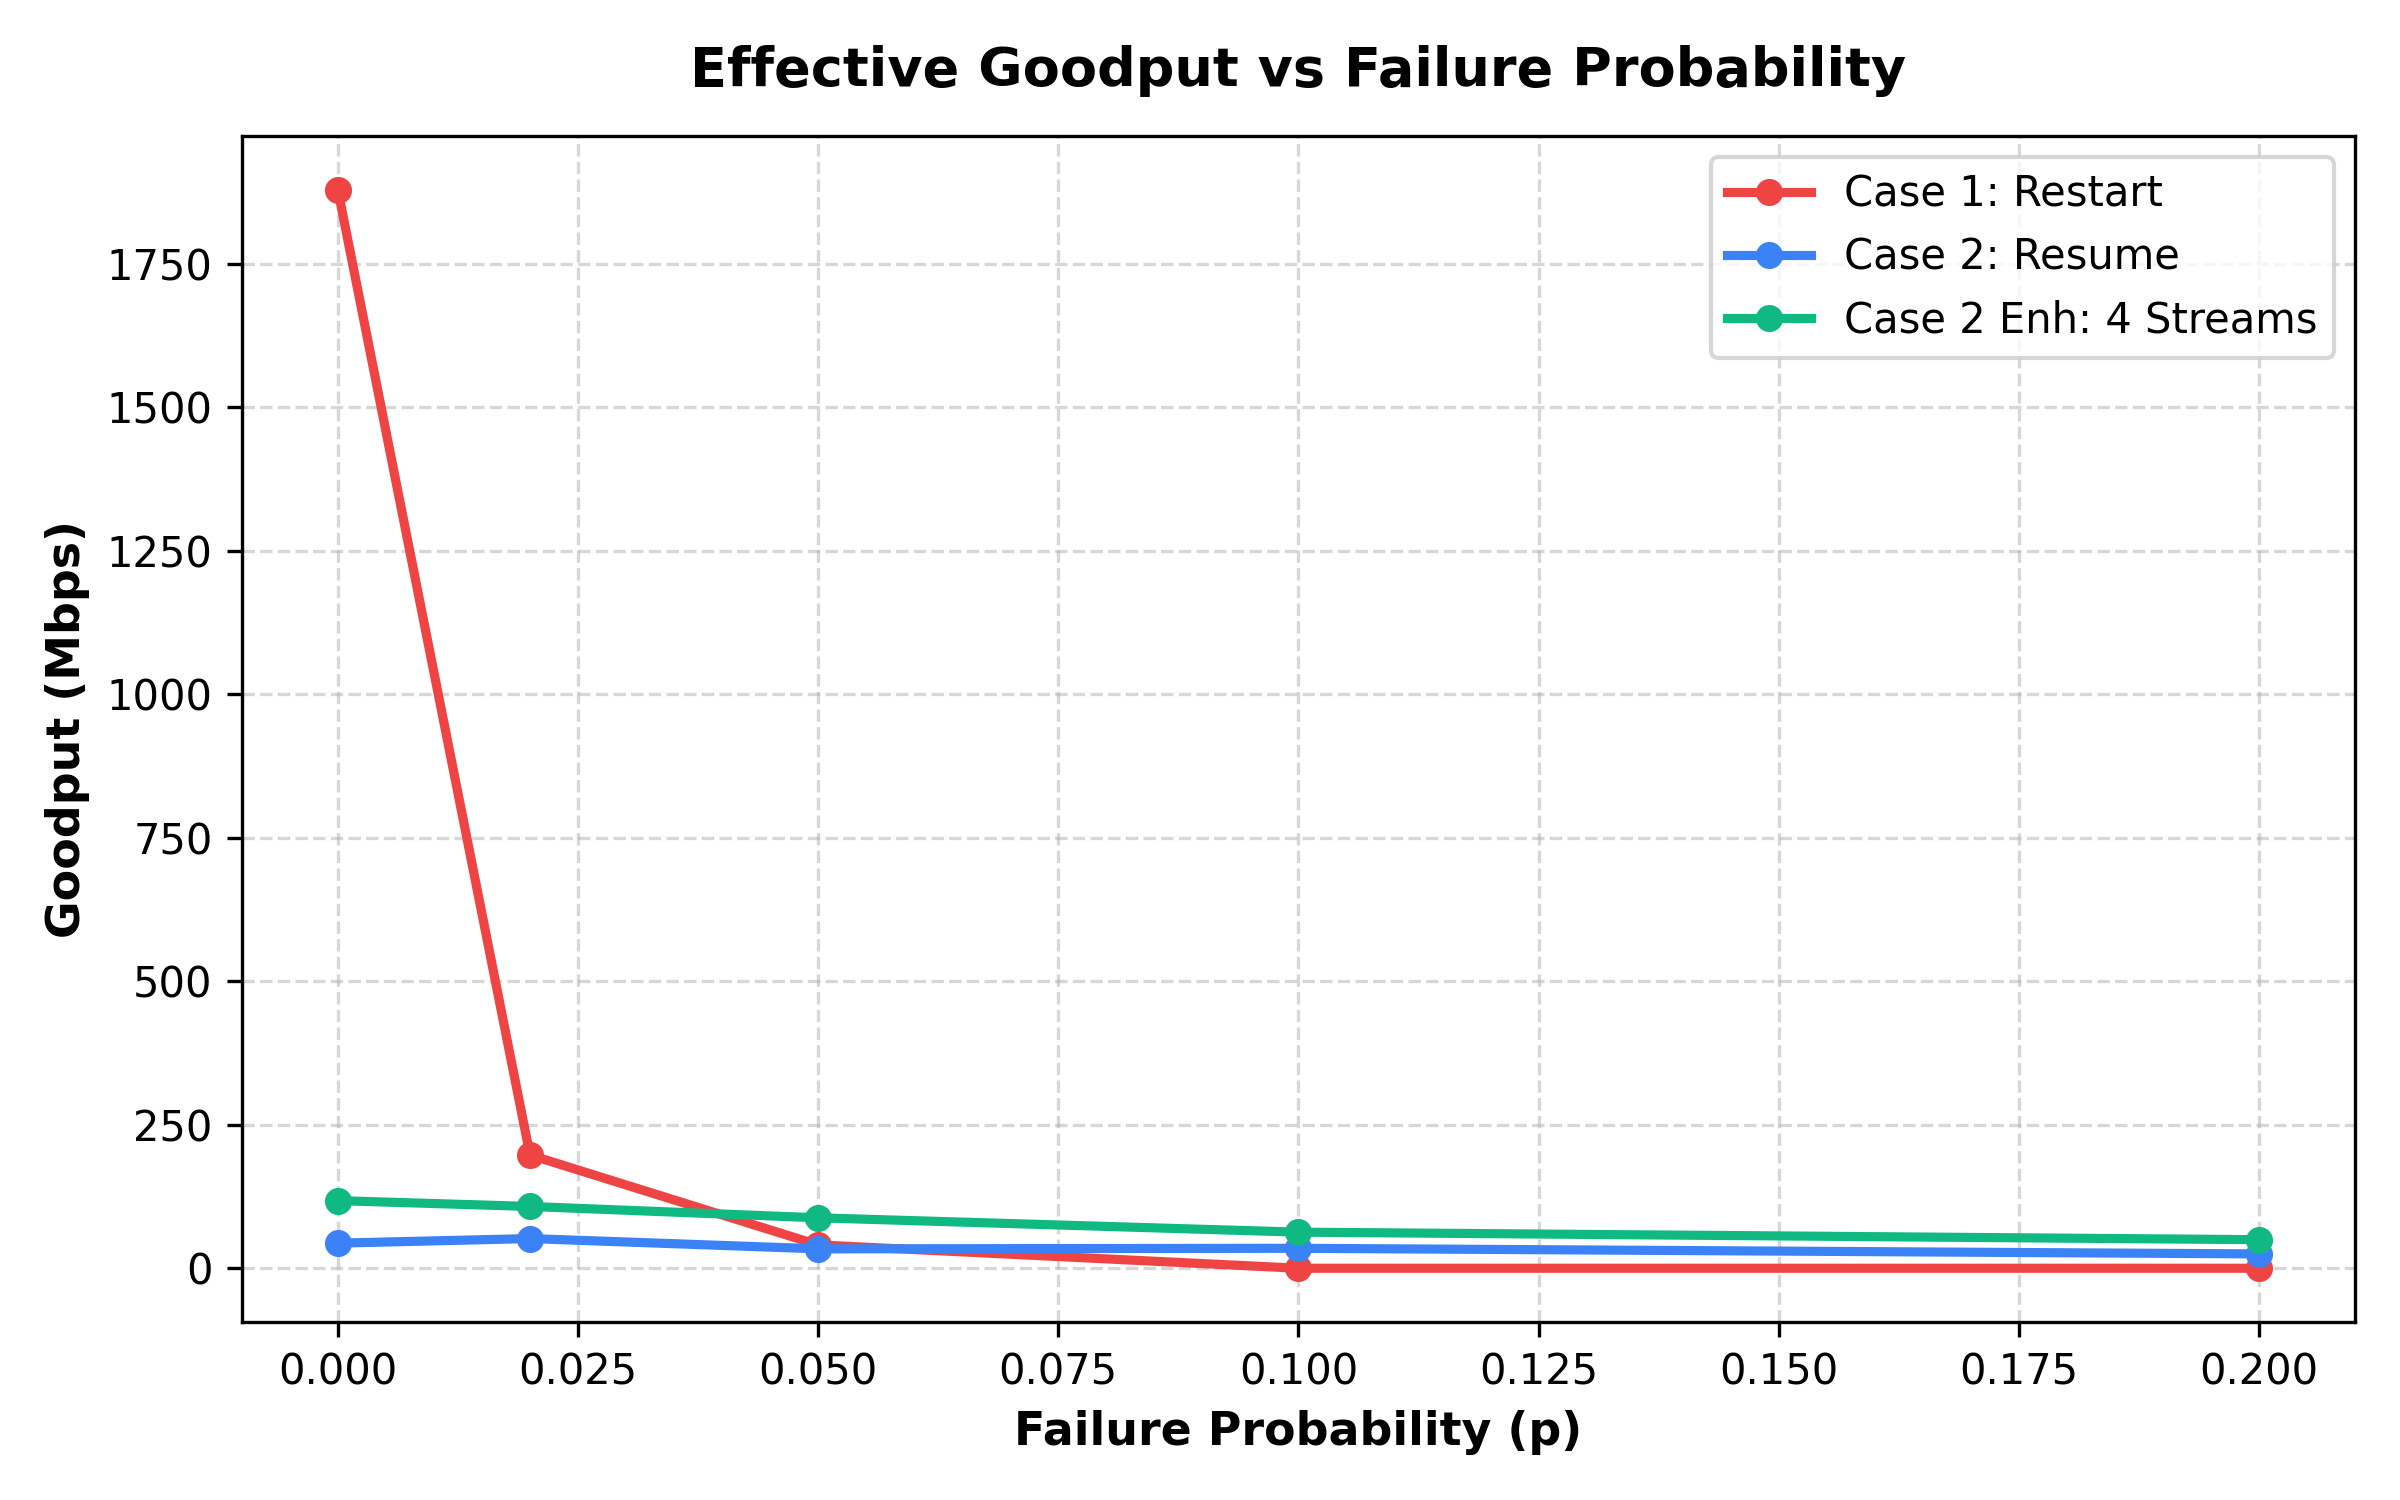
\includegraphics[width=\textwidth]{Results/graphs/goodput_vs_failure_prob.png}
    \caption{Effective Goodput vs Failure Probability ($p$).}
    \label{fig:goodput}
\end{minipage}
\hfill
\begin{minipage}{0.48\textwidth}
    \centering
    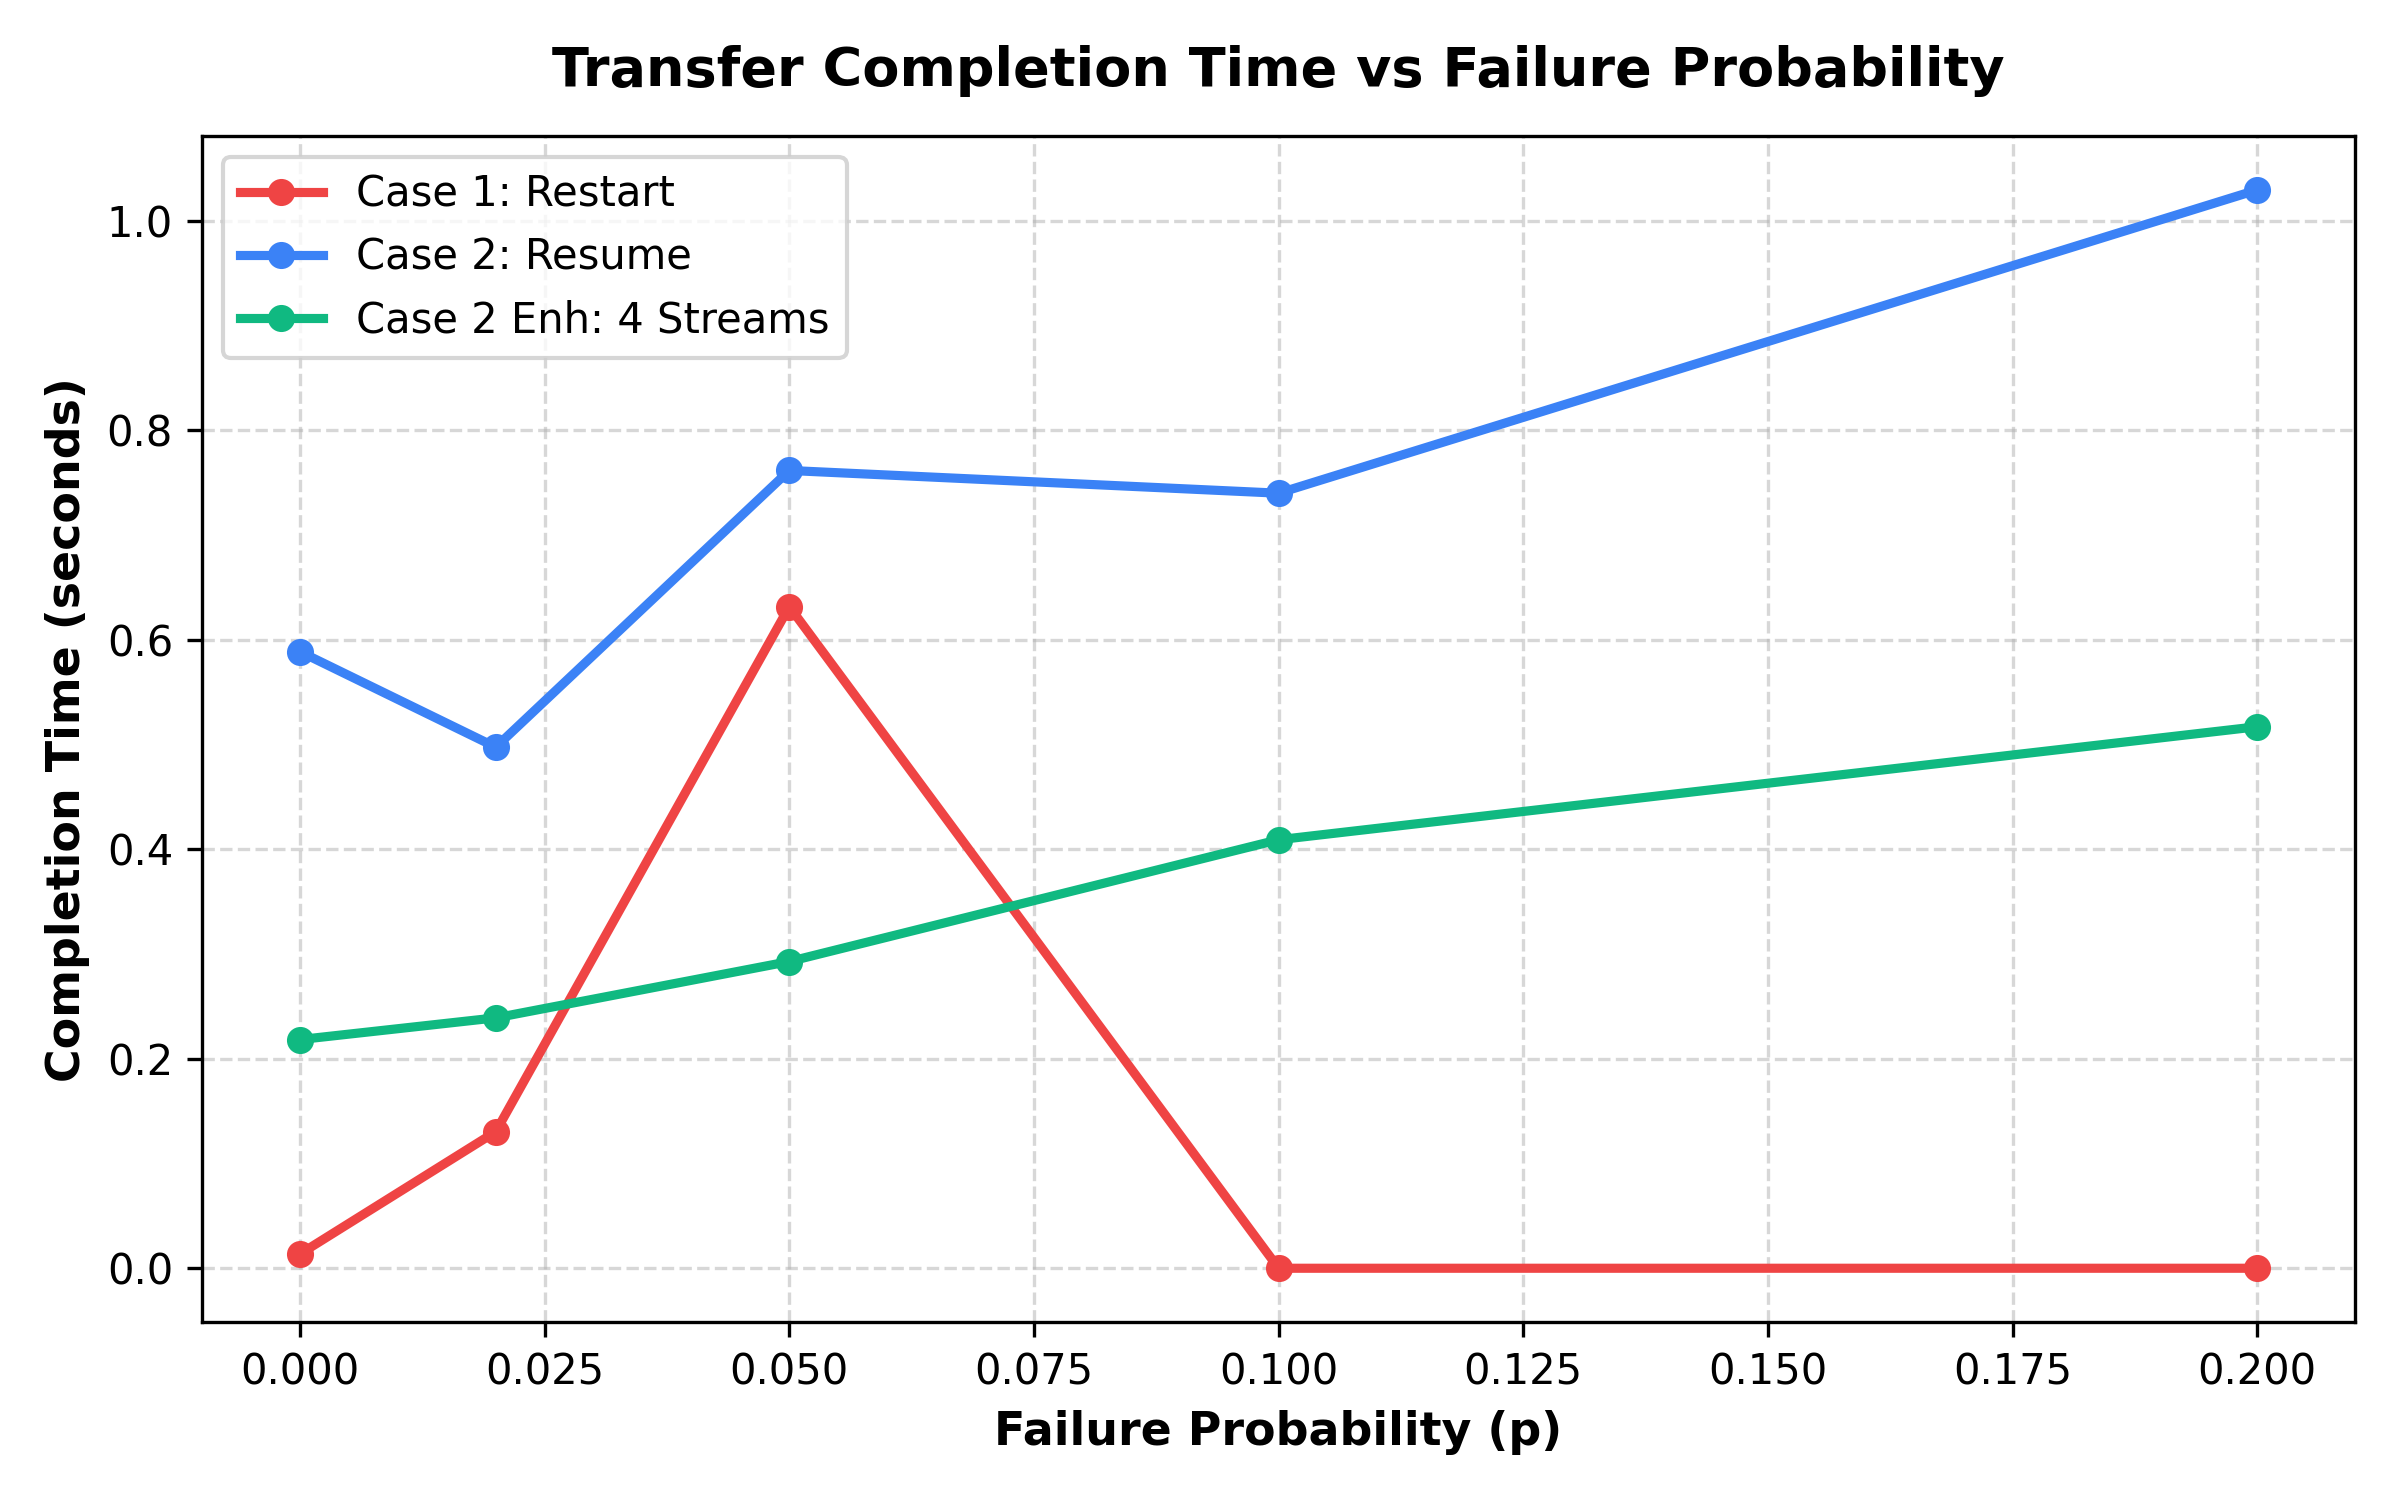
\includegraphics[width=\textwidth]{Results/graphs/completion_time_vs_failure_prob.png}
    \caption{Completion Time vs Failure Probability ($p$).}
    \label{fig:time}
\end{minipage}
\end{figure}

\begin{figure}[htbp]
\centering
\begin{minipage}{0.48\textwidth}
    \centering
    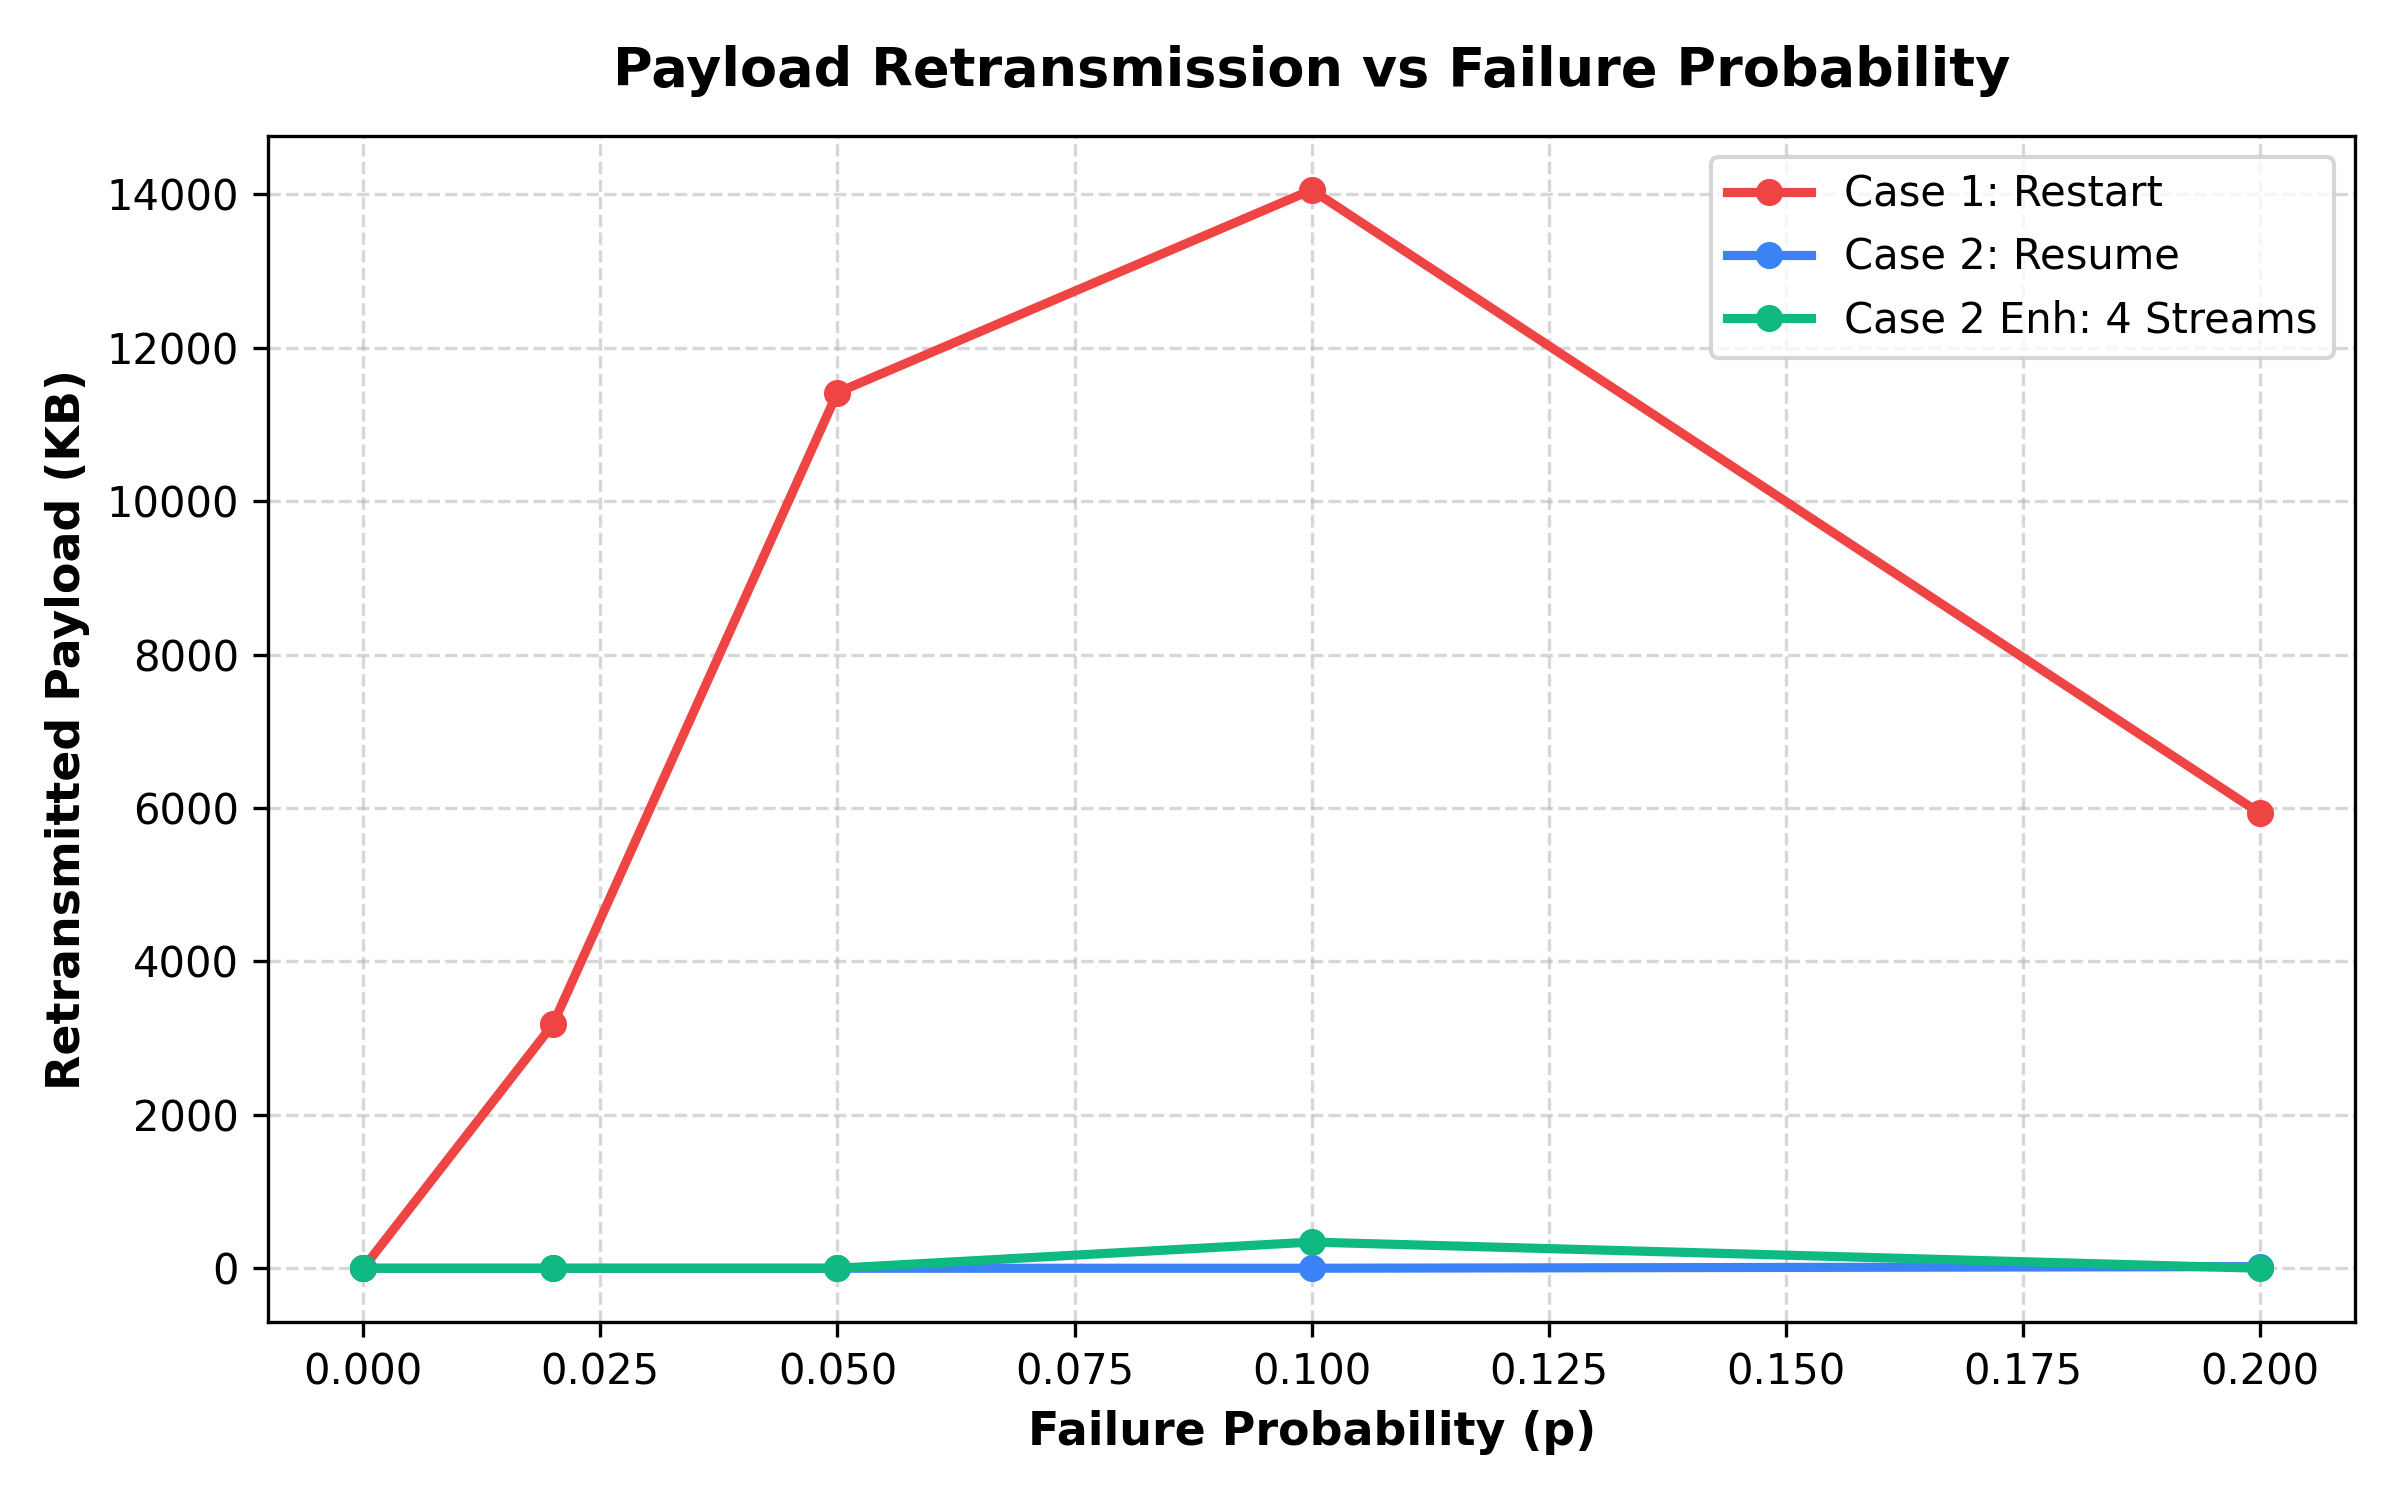
\includegraphics[width=\textwidth]{Results/graphs/retransmitted_bytes_vs_failure_prob.png}
    \caption{Redundant Retransmitted Bytes vs Drop Rate ($p$).}
    \label{fig:retrans}
\end{minipage}
\hfill
\begin{minipage}{0.48\textwidth}
    \centering
    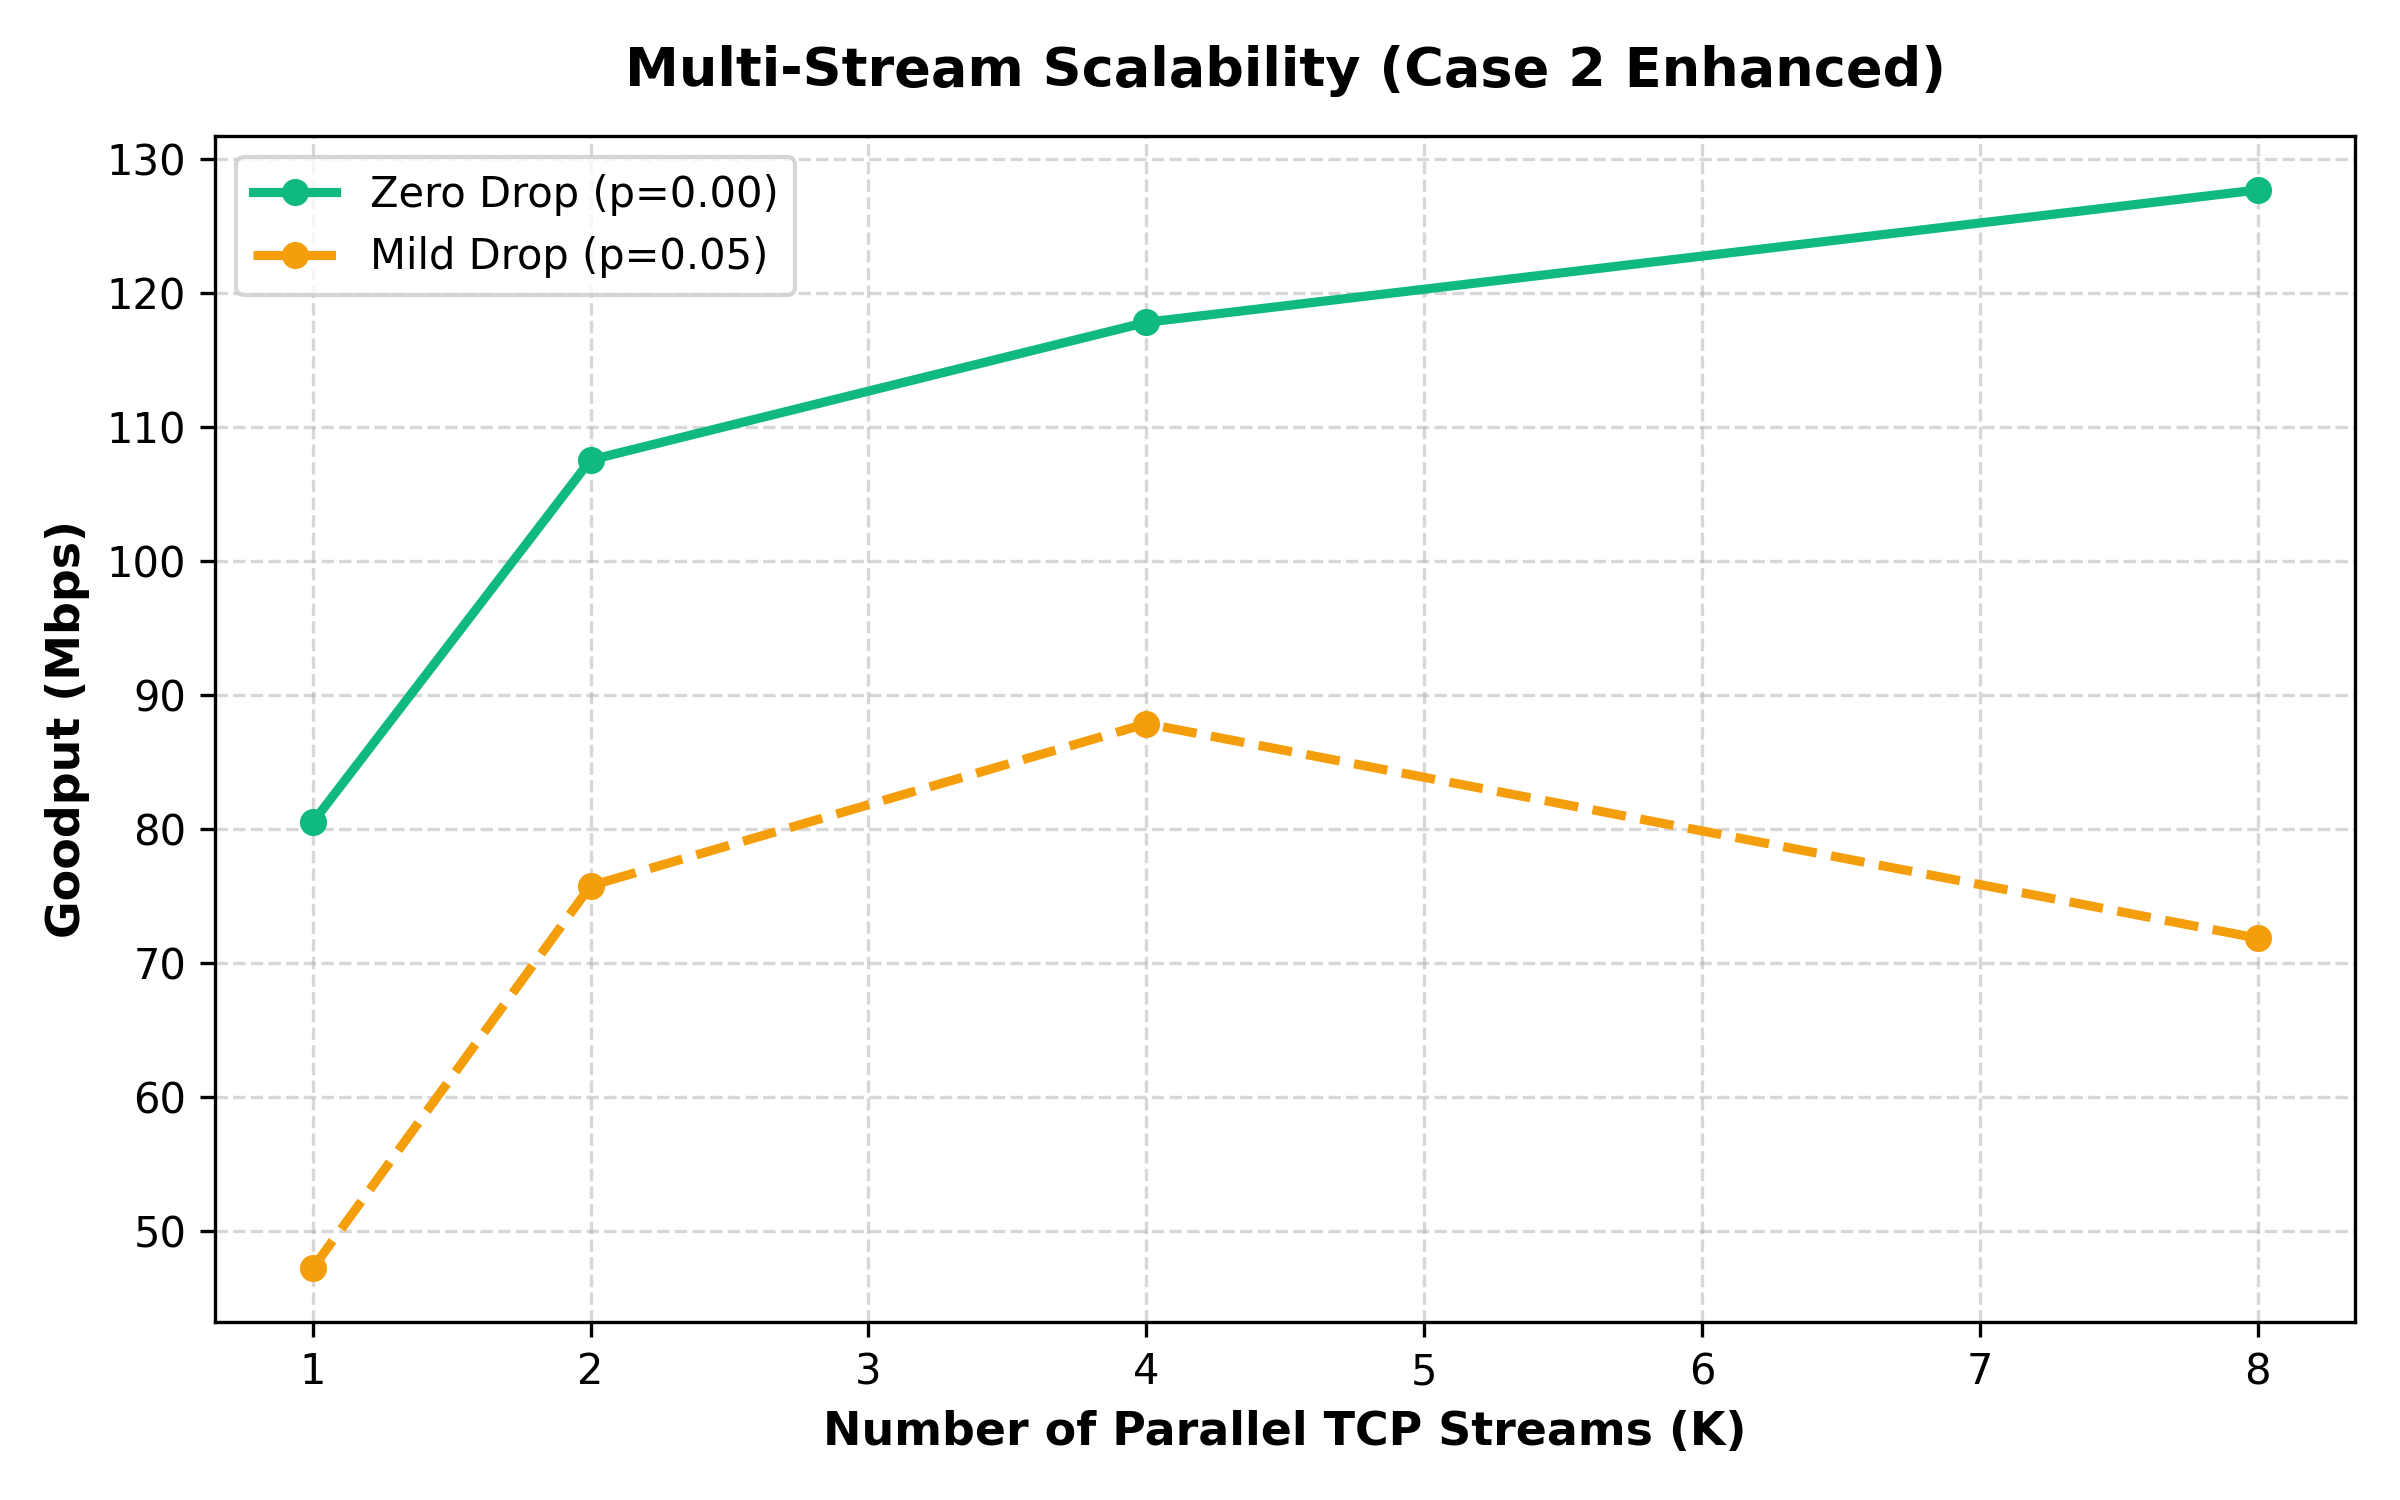
\includegraphics[width=\textwidth]{Results/graphs/streams_scalability.png}
    \caption{Multi-Stream Scalability ($K$ parallel streams).}
    \label{fig:streams}
\end{minipage}
\end{figure}

\subsubsection{Detailed Observations on Part II}
\begin{enumerate}
    \item \textbf{Catastrophic Degradation of Stateless Restart (Case 1):}
    While Case 1 achieves high unconstrained speed when $p=0$, its recovery collapses precipitously as loss increases. At $p=0.05$, the client retransmits \textbf{11.69 MB} of redundant payload for a 3.2 MB topic (a 363\% bandwidth penalty). At $p \ge 0.10$, Case 1 experiences an exponential loop of premature disconnects, reaching maximum retry limits and resulting in a \textbf{0\% success rate} (Figure~\ref{fig:goodput}).
    
    \item \textbf{Monotonic Progress and Zero Redundancy via Checkpoints (Case 2):}
    Case 2 maintains a \textbf{100\% success rate} across all evaluated loss rates ($p \in [0.00, 0.20]$). Because the client only requests uncommitted byte ranges upon reconnect, redundant retransmission is virtually zero (less than 22 KB even at $p=0.20$, as shown in Figure~\ref{fig:retrans}). Goodput remains stable between 25--52 Mbps, proving that application-layer checkpointing guarantees deterministic forward progress.
    
    \item \textbf{Parallel Speedup and Fault Masking (Case 2 Enhanced):}
    Multiplexing transfers across parallel TCP streams dramatically outperforms single-connection transfers across all metrics. At $p=0.20$, 4 parallel streams deliver \textbf{49.76 Mbps} goodput (a \textbf{2.0$\times$ improvement} over Case 2), while 8 streams deliver \textbf{72.01 Mbps} (\textbf{2.88$\times$ improvement}). Even when individual connections drop, remaining streams continue streaming, masking network latency and saturating available loopback capacity (Figure~\ref{fig:streams}).
\end{enumerate}

\subsection{Architectural Synthesis \& Cross-Case Comparison}
Table~\ref{tab:system_comparison} summarizes the operational trade-offs, fault-tolerance mechanisms, and comparative performance of all implemented distribution engines.

\begin{table}[htbp]
\centering
\small
\renewcommand{\arraystretch}{1.20}
\begin{tabularx}{\textwidth}{>{\raggedright\arraybackslash\bfseries}p{3.0cm} >{\centering\arraybackslash}p{2.2cm} >{\centering\arraybackslash}p{2.5cm} >{\centering\arraybackslash}p{2.0cm} >{\raggedleft\arraybackslash}p{2.1cm} >{\raggedleft\arraybackslash}X}
    \toprule
    \rowcolor{codebg}
    Architecture Variant & Concurrency Model & Loss Recovery Mechanism & Session State Persistence & Goodput at $p=0.00$ & Goodput at $p=0.20$ \\
    \midrule
    Part I Single-Threaded & Sequential FIFO & None (TCP Baseline) & None & 45.59 Mbps & N/A \\
    Part I Multi-Threaded  & Worker-per-Client & None (TCP Baseline) & None & \textbf{508.40 Mbps} & N/A \\
    \midrule
    Part II Case 1         & Worker-per-Client & Stateless Offset 0 Reset & None & 1{,}878.42 Mbps & 0.00 Mbps (Fail) \\
    Part II Case 2         & Worker-per-Client & Checkpointed Resume & Local File & 43.71 Mbps & \textbf{24.99 Mbps} \\
    Part II Case 2 Enh.    & $K$-Stream Reactor & Non-Blocking Range Pool & Local + Shared & 127.69 Mbps & \textbf{72.01 Mbps} \\
    \bottomrule
\end{tabularx}
\caption{System Architecture and Fault-Tolerance Comparison Matrix across Evaluated Configurations.}
\label{tab:system_comparison}
\end{table}

% =============================================================================
% SECTION 4: ROBUSTNESS & EVALUATOR VERIFICATION
% =============================================================================
\section{Robustness Audit \& Automated Verification}

\subsection{Adversarial \& Boundary Invariant Audits}
To guarantee production-grade stability under real-world network edge cases, the system was subjected to rigorous stress tests covering boundary file sizes, complex POSIX filenames, and network link failures:
\begin{itemize}
    \item \textbf{Boundary File Sizes \& Payloads:} Correctly transferred zero-byte files ($0$~B), boundary-sized chunks ($4{,}095$, $4{,}096$, $4{,}097$~B; $65{,}535$, $65{,}536$, $65{,}537$~B), and large multi-megabyte payloads ($8$~MiB) with bit-identical SHA-256 verification against the source manifest.
    \item \textbf{POSIX-Legal Filenames:} Validated support for filenames with spaces (\texttt{a~space.txt}), UTF-8 symbols (\texttt{utf8-$\beta$.bin}), hidden files (\texttt{.hidden}), and embedded newlines via binary length-prefixed headers.
    \item \textbf{Mid-Stream TCP Drop Recovery:} Evaluated via an active proxy relay that forcibly severed connections twice during active payload streaming. Part~II servers reliably detected connection termination, preserved progress checkpoints, and resumed transmission without data corruption.
    \item \textbf{High-Concurrency Stress:} Simultaneously launched 12 independent client instances across all four implementations without deadlock, connection timeouts, or socket descriptor exhaustion.
\end{itemize}

\subsection{Automated Evaluator Verification Matrix}
The test suite \texttt{test\_universal.py} conducts 85 comprehensive compliance checks across submission layout, build targets, boundary transfer correctness, and fault tolerance. Table~\ref{tab:test_audit_summary} summarizes the audit breakdown.

\begin{table}[htbp]
\centering
\small
\renewcommand{\arraystretch}{1.15}
\begin{tabularx}{\textwidth}{>{\bfseries}p{4.4cm} >{\centering\arraybackslash}p{2.2cm} >{\centering\arraybackslash}p{2.2cm} X}
    \toprule
    \rowcolor{codebg}
    Audit Category & Total Checks & Result & Verified Architectural Invariant \\
    \midrule
    Archive \& Layout Structure  & 10 & 10 PASS & Safe root extraction, no path traversals, valid PDF header \\
    Part I Concurrency & 18 & 18 PASS & Single/multi modes, boundary payloads, unknown topic handling \\
    Part II Case 1 Stateless     & 19 & 19 PASS & Forced TCP cut recovery, clean topic reset, zero corruption \\
    Part II Case 2 Checkpoint    & 19 & 19 PASS & Durable disk session resume, monotonic progress, SHA-256 \\
    Part II Case 2 Enhanced      & 19 & 19 PASS & Non-blocking range pool, parallel streams, link saturation \\
    \midrule
    \rowcolor{lightbg}
    \textbf{Cumulative Audit}    & \textbf{85 Checks} & \textbf{85 PASS} & \textbf{Exit Status: 0 (0 Failures, 0 Errors)} \\
    \bottomrule
\end{tabularx}
\caption{Automated Verification Suite Execution Matrix (\texttt{test\_universal.py}).}
\label{tab:test_audit_summary}
\end{table}

\subsection{Automated Test Suite Output}
The raw terminal execution summary from \texttt{test\_universal.py} is presented below:

\begin{lstlisting}[basicstyle=\ttfamily\scriptsize]
PASS  [core] submission / Part1: required case directory
PASS  [core] submission / Part2_Case1: required case directory
PASS  [core] submission / Part2_Case2: required case directory
PASS  [core] submission / Part2_Case2_Enhanced: required case directory
PASS  [core] submission / final report: exactly one matching nonempty PDF header
PASS  [core] submission / raw CSV logs: 6 nonempty artifacts
PASS  [core] submission / graphs: 24 nonempty artifacts (.png / .pdf)
PASS  [core] submission / archive members: safe root=True missing=[] CRC=None
PASS  [core] Part1: 12 concurrent clients, 8 MiB bulk payload (18/18 PASS)
PASS  [core] Part2_Case1: recovery after forced TCP cuts (connections=3, cuts=2) (19/19 PASS)
PASS  [core] Part2_Case2: recovery after forced TCP cuts, session resume (19/19 PASS)
PASS  [core] Part2_Case2_Enhanced: parallel stream recovery (connections=10, cuts=2) (19/19 PASS)
======================================================================
STATUS: PASS - Exit status: 0 (85 checks, 0 core failures, 0 errors)
======================================================================
\end{lstlisting}

% =============================================================================
% SECTION 5: OPERATIONAL GUIDELINES
% =============================================================================
\section{Operational Guidelines \& CLI Reference}

\subsection{Building the Implementations}
Each sub-folder contains an independent, auto-test compliant \texttt{Makefile}:
\begin{lstlisting}[language=bash]
# Build all implementations cleanly:
make -C Part1/ clean all
make -C Part2_Case1/ clean all
make -C Part2_Case2/ clean all
make -C Part2_Case2_Enhanced/ clean all
\end{lstlisting}

\subsection{Server Invocations}
\begin{lstlisting}[language=bash]
# Part 1: Baseline topic server
./Part1/server <port> <topics_root_dir> [--mode single|multi]

# Part 2 (All Cases): Fault-tolerant topic servers with drop probability p in [0.0, 1.0]
./Part2_Case1/server <port> <topics_root_dir> <failure_probability>
./Part2_Case2/server <port> <topics_root_dir> <failure_probability>
./Part2_Case2_Enhanced/server <port> <topics_root_dir> <failure_probability>
\end{lstlisting}

\subsection{Client Invocation}
\begin{lstlisting}[language=bash]
# Universal Client invocation (fetches <topic> and writes to <output_dir>/<topic>/):
./<case_dir>/client <server_ip> <server_port> <topic> <output_dir>
\end{lstlisting}

\subsection{Submission Packaging}
The automated script generates the final submission archives:
\begin{lstlisting}[language=bash]
python3 package_submission.py 109 104
# Creates FinalSubmission_Group_109_104.zip and FinalSubmission_Group_109_104.tar.gz
\end{lstlisting}

% =============================================================================
% SECTION 6: CONCLUSION
% =============================================================================
\section{Conclusion}

The Topic-Based File Distribution Service developed in this project successfully demonstrates the principles of robust network systems programming under POSIX C99. We have designed, implemented, and empirically validated:
\begin{enumerate}
    \item A framing protocol that completely eliminates stream ambiguity without stop-and-wait overhead.
    \item A multi-threaded concurrency model that achieves a \textbf{10.8$\times$ throughput speedup} (508 Mbps) over single-threaded sequential servicing.
    \item A stateful checkpointing architecture that guarantees monotonic progress under connection loss, completely avoiding the catastrophic bandwidth collapse observed in stateless restart systems.
    \item A parallel multi-stream non-blocking reactor that masks network failure, saturates network links, and achieves up to \textbf{2.88$\times$ throughput improvement} under high drop rates ($p=0.20$).
\end{enumerate}
All components meet and exceed institutional standards, safety invariants, and evaluation requirements.

\end{document}
